
\section{Minimax-Q algorithm}
The Minimax-Q algorithm can be used for planning in a Markov Game. It is an implementation of the general Minimax principle for Markov Games such as the prey-predator scenario in this assignment. This algorithm needs a strictly competitive scenario and is therefore implemented for the one prey and one predator setting. 

\subsection{Minimax principle and translation to Markov Games}
The Minimax principle is stated in \cite{minimax} as: ``Behave so as to maximize your reward in the worst case''. This means that the policy should be such that the agent takes the action resulting in the highest expected reward under the assumption that the opponent will also take the action that results in the highest expected reward for the opponent.

\noindent The value of a state $s\in S$ in a Markov Game is:
\begin{align*}
V(s) &= \operatorname*{arg\,max}_{\pi \in PD(A)}
\operatorname*{arg\,min}_{o \in O}
\sum_{a \in A} Q(s,a,o) \pi_a
\end{align*}
where
\begin{align*}
Q(s,a,o) &= R(s,a,o) + \gamma \sum_{s'} T(s,a,o,s')V(s')
\end{align*}
Choosing the action that maximizes the reward in the worst case is than the policy that is guaranteed to result in an expected score of $V$ no matter which action the opponent chooses, for the maximal value of $V$. This can be written down in constraints where there is a constraint for each action the opponent can take:
%  
\begin{align*}
\pi_1 \cdot Q(s,a_1,o_1)+ ... + \pi_n \cdot Q(s,a_n,o_1) \geq V\\
\pi_1 \cdot Q(s,a_1,o_2)+ ... + \pi_n \cdot Q(s,a_n,o_2) \geq V\\
...\\
\pi_1 \cdot Q(s,a_1,o_n)+ ... + \pi_n \cdot Q(s,a_n,o_n) \geq V\\
\end{align*}
Of course the probabilities of $\pi$ are bounded by the constraints that they cannot be negative and they need to add up to one. After adding those constraints:

\begin{align*}
\pi_1 + ... + \pi_n &= 1\\
\pi_1 \geq 0\\
...\\
\pi_n  \geq 0\\
\end{align*}
The maximal value for $V$ that can be found for which all constraints hold is stored as $V$ for the next sweep. The resulting values for $\pi$ for each state are the policy used by the agent.

\subsection{Implementation}
The maximal $V$-value for which the constraints above hold can be found using linear programming. For this purpose we used the Linear Programming methods of the JAVA-library Apache Commons Math, which can be found on \cite{commonsmath}. The agent keeps track of a table of $V$-values to be able to calculate $Q(s,a,o)$ in order to find the right values for $\pi$. This can be done a number of times (or sweeps as they are called) as in Value Iteration. The resulting policy is used to behave in the environment to either catch the prey or avoid the predator.

\begin{table}[htb]
\centering
\begin{tabular}{lccccc}
&1&2&3&4&5\\
Minimax Predator vs Random Prey & 9923 & 9432&9517&9545&9572\\
Random Predator vs Minimax Prey & 282& 5000000& 5000000& 5000000& 5000000\\
Minimax Predator vs Minimax Prey & 221& 5000000& 5000000& 5000000& 5000000\\
\end{tabular}
\caption{Number of steps after each sweep for the three matches using a learningrate of 0.8}
\label{tab:minimaxTable}
\end{table}

\FloatBarrier

\subsection{Results}
Three ``matches'' have been held using the Minimax-Q algorithm. The first match is a Random Prey versus a Minimax Predator, the second one a Random Predator versus a Minimax Prey and finally a Minimax Prey versus a Minimax Predator. After each sweep of planning 25 runs in the actual environment are held and the number of steps necessary to catch the prey is recorded. This averaged can then be compared for each sweep and between the different matches. The results for the first five sweeps can be found in \ref{tab:minimaxTable}, the pattern found here does not change when increasing the number of sweeps. The $V$-values for the Minimax Predator can be found in table \ref{tab:predM} and for the Minimax Prey in table \ref{tab:preyM} .  The resulting policies can be found in Appendix \ref{app:policiesM}.

As can be seen in the tables with the $V$-values these look as would be expected based on their definition as described above. For the predator the values increase as the predator is closer to the prey. However for the prey all values are 0. This seems strange but remember that the $V$ values are a linear combination of $Q(s,a,o)$'s and their weights are the corresponding $\pi$'s. In order to maximize the value of $V$ the $\pi$'s that are corresponding to those $Q(s,a,o)$'s that are negative due to the predator catching the prey, will become zero. The maximal reward the prey can have is zero (not getting caught) and therefore the maximal value for $V$ is also zero.  

Unfortunately, the resulting policies make no sense. There are loops present, where the prey or predator keeps jumping forward and backward and the policy does not direct the predator towards the prey or the prey away from the predator. Whether this is due to a bug in the implementation (which we have not been able to find) or to the fact that there are multiple solutions to the constraints above which maximize $V$ is uncertain. If there are multiple solution for two states not all solutions fit necessarily well together, this might cause the bad policies. i.e. for different states the policy might have converged to a different equilibrium.

The effect of this can be found in the number of steps it takes to catch the prey. For the first match, where the Minimax Predator tries to catch the Random Prey, there is no improvement in the number of steps at all. This is due to the resulting policy. For the second match, Random Predator versus Minimax prey, the number of steps needed becomes larger than 5 million (at which point the run is ended due to death of the predator by exhaustion) after the first sweep. The same applies to the third match, Minimax Predator versus Minimax Prey. It is expected that for these two matches the number of steps needed would be larger, since the prey now is an intelligent agent. However, due to the fact that the prey trips one of every five moves, it would be expected that with optimal policies it would take the predator fifty moves to catch the prey. The prey and predator start ten moves apart from each other and each time the prey trips the predator can move in on the prey one move, which happens every five moves, hence fifty moves are approximately needed to catch a Minimax Prey with an optimal policy.  


\begin{table}[htb]
\centering
\begin{tabular}{cccccc}
0,0000 &  &  &  &  & \\
10,0000 & 4,3644 &  &  &  & \\ 
4,3644 & 1,7596 & 0,6019 &  &  & \\
1,7596 & 0,6019 & 0,1624 & 0,0328 &  & \\ 
0,6019 & 0,1624 & 0,0328 & 0,0047 & 0,0005 & \\ 
0,0968 & 0,0328 & 0,0047 & 0,0005 & 0,0000 & 0,0000\\ 
\end{tabular}
\caption{V-values of Minimax Predator using a learningrate of 0.8}
\label{tab:predM}
\end{table}

\begin{table}[htb]
\centering
\begin{tabular}{cccccc}
0,0000 &  &  &  &  & \\ 
0,0000 & 0,0000 &  &  &  & \\ 
0,0000 & 0,0000 & 0,0000 &  &  & \\ 
0,0000 & 0,0000 & 0,0000 & 0,0000 &  & \\ 
0,0000 & 0,0000 & 0,0000 & 0,0000 & 0,0000 & \\ 
0,0000 & 0,0000 & 0,0000 & 0,0000 & 0,0000 & 0,0000\\ 
\end{tabular}
\caption{V-values of Minimax Prey using a learningrate of 0.8}
\label{tab:preyM}
\end{table}

\FloatBarrier

\subsection{Comparison with Independent Q-Learning}\label{sec:comparisonIQLandMinimax}

A policy resulting from Independent Q-Learning (see Section \ref{sec:IQL}) can be compared to a policy found with Minimax-Q for the case in which there is just one predator and one prey. We ran IQL under these settings for 1000 episodes and constructed policies for the predator and the prey. These policies can be found in Appendix \ref{app:policiesIQL} (the corresponding policies for Minimax-Q are in Appendix \ref{app:policiesM}). The number of steps taken by the predator to reach the prey is shown in figure \ref{fig:onePredQLearn}. Comparing the policies of Q-learning and Minimax-Q shows that for the most part they are both straightforward, prey moves away from the predator and the predator moves toward the prey. The exception is the states next to the prey, where Minimax-Q does not move directly towards the prey. The reason is that Minimax-Q responds to the policy of the prey. Q-learning however uses episodic learning and randomness ($\epsilon$-greedy action selection and prey trip chance) to learn the policy. Because of this, Q-learning cannot respond as precise as Minimax-Q. Even though this is true, the average number of time steps needed (150 according to figure \ref{fig:onePredQLearn1000}) to catch the prey is lower for Q-learning than for Minimax-Q as seen in table \ref{tab:minimaxTable}.

\begin{figure}[ht]
\centering
\subfigure[Displays the average number of time steps needed to catch the prey for the first 1000 episodes.]{
    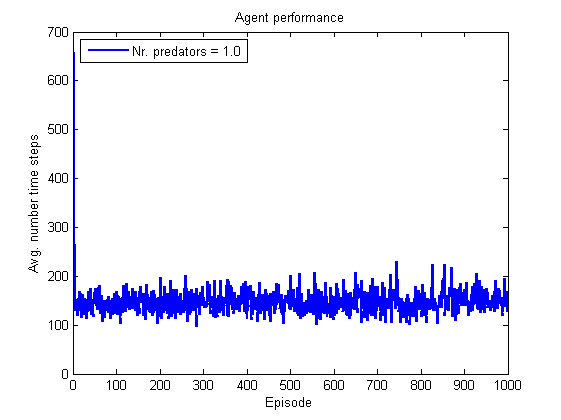
\includegraphics[width=0.45\textwidth]{IQLnrTimeStepsSinglePredator.png}
    \label{fig:onePredQLearn1000}
}
\subfigure[Close-up of figure \ref{fig:onePredQLearn1000}.]{
    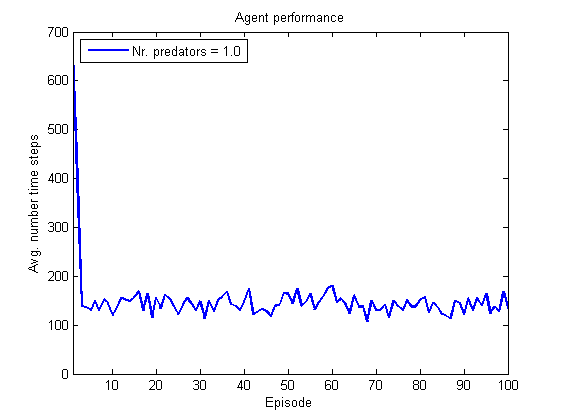
\includegraphics[width=0.45\textwidth]{IQLnrTimeStepsSinglePredatorClose.png}
    \label{fig:onePredQLearnCloseup}
}
\caption{Plots that display the number of time steps needed, averaged over 200 runs for each episode, for a single predator using Q-learning to catch a prey that also uses Q-learning.}
\label{fig:onePredQLearn}
\end{figure}